\documentclass[twoside]{book}

% Packages required by doxygen
\usepackage{calc}
\usepackage{doxygen}
\usepackage{graphicx}
\usepackage[utf8]{inputenc}
\usepackage{makeidx}
\usepackage{multicol}
\usepackage{multirow}
\usepackage{textcomp}
\usepackage[table]{xcolor}

% NLS support packages
\usepackage[french]{babel}

% Font selection
\usepackage[T1]{fontenc}
\usepackage{mathptmx}
\usepackage[scaled=.90]{helvet}
\usepackage{courier}
\usepackage{amssymb}
\usepackage{sectsty}
\renewcommand{\familydefault}{\sfdefault}
\allsectionsfont{%
  \fontseries{bc}\selectfont%
  \color{darkgray}%
}
\renewcommand{\DoxyLabelFont}{%
  \fontseries{bc}\selectfont%
  \color{darkgray}%
}

% Page & text layout
\usepackage{geometry}
\geometry{%
  a4paper,%
  top=2.5cm,%
  bottom=2.5cm,%
  left=2.5cm,%
  right=2.5cm%
}
\tolerance=750
\hfuzz=15pt
\hbadness=750
\setlength{\emergencystretch}{15pt}
\setlength{\parindent}{0cm}
\setlength{\parskip}{0.2cm}
\makeatletter
\renewcommand{\paragraph}{%
  \@startsection{paragraph}{4}{0ex}{-1.0ex}{1.0ex}{%
    \normalfont\normalsize\bfseries\SS@parafont%
  }%
}
\renewcommand{\subparagraph}{%
  \@startsection{subparagraph}{5}{0ex}{-1.0ex}{1.0ex}{%
    \normalfont\normalsize\bfseries\SS@subparafont%
  }%
}
\makeatother

% Headers & footers
\usepackage{fancyhdr}
\pagestyle{fancyplain}
\fancyhead[LE]{\fancyplain{}{\bfseries\thepage}}
\fancyhead[CE]{\fancyplain{}{}}
\fancyhead[RE]{\fancyplain{}{\bfseries\leftmark}}
\fancyhead[LO]{\fancyplain{}{\bfseries\rightmark}}
\fancyhead[CO]{\fancyplain{}{}}
\fancyhead[RO]{\fancyplain{}{\bfseries\thepage}}
\fancyfoot[LE]{\fancyplain{}{}}
\fancyfoot[CE]{\fancyplain{}{}}
\fancyfoot[RE]{\fancyplain{}{\bfseries\scriptsize Généré le Dimanche 25 Mai 2014 13\-:02\-:10 pour Bataille Navale par Doxygen }}
\fancyfoot[LO]{\fancyplain{}{\bfseries\scriptsize Généré le Dimanche 25 Mai 2014 13\-:02\-:10 pour Bataille Navale par Doxygen }}
\fancyfoot[CO]{\fancyplain{}{}}
\fancyfoot[RO]{\fancyplain{}{}}
\renewcommand{\footrulewidth}{0.4pt}
\renewcommand{\chaptermark}[1]{%
  \markboth{#1}{}%
}
\renewcommand{\sectionmark}[1]{%
  \markright{\thesection\ #1}%
}

% Indices & bibliography
\usepackage{natbib}
\usepackage[titles]{tocloft}
\setcounter{tocdepth}{3}
\setcounter{secnumdepth}{5}
\makeindex

% Hyperlinks (required, but should be loaded last)
\usepackage{ifpdf}
\ifpdf
  \usepackage[pdftex,pagebackref=true]{hyperref}
\else
  \usepackage[ps2pdf,pagebackref=true]{hyperref}
\fi
\hypersetup{%
  colorlinks=true,%
  linkcolor=blue,%
  citecolor=blue,%
  unicode%
}

% Custom commands
\newcommand{\clearemptydoublepage}{%
  \newpage{\pagestyle{empty}\cleardoublepage}%
}


%===== C O N T E N T S =====

\begin{document}

% Titlepage & ToC
\hypersetup{pageanchor=false}
\pagenumbering{roman}
\begin{titlepage}
\vspace*{7cm}
\begin{center}%
{\Large Bataille Navale \\[1ex]\large 0.\-1 }\\
\vspace*{1cm}
{\large Généré par Doxygen 1.8.6}\\
\vspace*{0.5cm}
{\small Dimanche 25 Mai 2014 13:02:10}\\
\end{center}
\end{titlepage}
\clearemptydoublepage
\tableofcontents
\clearemptydoublepage
\pagenumbering{arabic}
\hypersetup{pageanchor=true}

%--- Begin generated contents ---
\chapter{Index des espaces de nommage}
\section{Liste des espaces de nommage}
Liste de tous les espaces de nommage avec une brève description\-:\begin{DoxyCompactList}
\item\contentsline{section}{\hyperlink{namespaceconstantes}{constantes} }{\pageref{namespaceconstantes}}{}
\item\contentsline{section}{\hyperlink{namespaceserveur}{serveur} }{\pageref{namespaceserveur}}{}
\end{DoxyCompactList}

\chapter{Index hiérarchique}
\section{Hiérarchie des classes}
Cette liste d'héritage est classée approximativement par ordre alphabétique \-:\begin{DoxyCompactList}
\item \contentsline{section}{serveur.\-Bat\-Nav}{\pageref{classserveur_1_1BatNav}}{}
\item \contentsline{section}{object}{\pageref{classobject}}{}
\begin{DoxyCompactList}
\item \contentsline{section}{map\-I\-A.\-bateau}{\pageref{classmapIA_1_1bateau}}{}
\end{DoxyCompactList}
\end{DoxyCompactList}

\chapter{Index des classes}
\section{Liste des classes}
Liste des classes, structures, unions et interfaces avec une brève description \-:\begin{DoxyCompactList}
\item\contentsline{section}{\hyperlink{classserveur_1_1BatNav}{serveur.\-Bat\-Nav} \\*Cette classe est la définition d'un service web }{\pageref{classserveur_1_1BatNav}}{}
\end{DoxyCompactList}

\chapter{Index des fichiers}
\section{Liste des fichiers}
Liste de tous les fichiers avec une brève description \-:\begin{DoxyCompactList}
\item\contentsline{section}{\hyperlink{bateau_8py}{bateau.\-py} }{\pageref{bateau_8py}}{}
\item\contentsline{section}{\hyperlink{constantes_8py}{constantes.\-py} \\*Copyright (c) 2014 Georges Khaznadar \href{mailto:georgesk@debian.org}{\tt georgesk@debian.\-org} }{\pageref{constantes_8py}}{}
\item\contentsline{section}{\hyperlink{mapIA_8py}{map\-I\-A.\-py} \\*Ce fichier fait partie du projet Batnav Batnav est un petit logiciel libre, vous avez le droit de le r�utiliser � votre convenance, dans le respect de la licence G\-P\-L V3, ou, selon vos pr�f�rences, de toute version ult�rieure de celle-\/ci }{\pageref{mapIA_8py}}{}
\item\contentsline{section}{\hyperlink{serveur_8py}{serveur.\-py} \\*Copyright (c) 2014 Georges Khaznadar \href{mailto:georgesk@debian.org}{\tt georgesk@debian.\-org} }{\pageref{serveur_8py}}{}
\end{DoxyCompactList}

\chapter{Documentation des espaces de nommage}
\hypertarget{namespacebateau}{\section{Référence de l'espace de nommage bateau}
\label{namespacebateau}\index{bateau@{bateau}}
}
\subsection*{Fonctions}
\begin{DoxyCompactItemize}
\item 
def \hyperlink{namespacebateau_a2f0e2fb6690af90fd1cd510e132a041c}{map}
\item 
def \hyperlink{namespacebateau_ad2ef327d271e5ebe5426fe6d58fa0cea}{Porte\-Avion}
\item 
def \hyperlink{namespacebateau_a472c5b7bcdfb78f0e7388a197a25129a}{Croiseur}
\item 
def \hyperlink{namespacebateau_a91714c8dcf7e649256b4abd289176d58}{Contre\-Torpilleur}
\item 
def \hyperlink{namespacebateau_ae08b97eef04ed71124cda74053ad0a36}{Sous\-Marin}
\item 
def \hyperlink{namespacebateau_a875c36de98747c833df6a8c648f0ced3}{Torpilleur}
\item 
def \hyperlink{namespacebateau_aa9dece4300bcd47e6e67cdaa52fa2cce}{sens}
\item 
def \hyperlink{namespacebateau_ad1217acc7738157178dae5d246b019db}{originex}
\item 
def \hyperlink{namespacebateau_a2b16dc7153e94407fdbb3c8d4a152a84}{originey}
\end{DoxyCompactItemize}
\subsection*{Variables}
\begin{DoxyCompactItemize}
\item 
tuple \hyperlink{namespacebateau_a924cee8dc4435fc03e905904c31dbcf7}{Carte\-Joueur} = \hyperlink{namespacebateau_a2f0e2fb6690af90fd1cd510e132a041c}{map}()
\item 
tuple \hyperlink{namespacebateau_a50dc5f1cd8aae1c80cfd24007c44dd9c}{Carte\-Adv} = \hyperlink{namespacebateau_a2f0e2fb6690af90fd1cd510e132a041c}{map}()
\end{DoxyCompactItemize}


\subsection{Documentation des fonctions}
\hypertarget{namespacebateau_a91714c8dcf7e649256b4abd289176d58}{\index{bateau@{bateau}!Contre\-Torpilleur@{Contre\-Torpilleur}}
\index{Contre\-Torpilleur@{Contre\-Torpilleur}!bateau@{bateau}}
\subsubsection[{Contre\-Torpilleur}]{\setlength{\rightskip}{0pt plus 5cm}def bateau.\-Contre\-Torpilleur (
\begin{DoxyParamCaption}
\item[{}]{sens, }
\item[{}]{originex, }
\item[{}]{originey}
\end{DoxyParamCaption}
)}}\label{namespacebateau_a91714c8dcf7e649256b4abd289176d58}


Définition à la ligne 74 du fichier bateau.\-py.

\hypertarget{namespacebateau_a472c5b7bcdfb78f0e7388a197a25129a}{\index{bateau@{bateau}!Croiseur@{Croiseur}}
\index{Croiseur@{Croiseur}!bateau@{bateau}}
\subsubsection[{Croiseur}]{\setlength{\rightskip}{0pt plus 5cm}def bateau.\-Croiseur (
\begin{DoxyParamCaption}
\item[{}]{sens, }
\item[{}]{originex, }
\item[{}]{originey}
\end{DoxyParamCaption}
)}}\label{namespacebateau_a472c5b7bcdfb78f0e7388a197a25129a}


Définition à la ligne 45 du fichier bateau.\-py.

\hypertarget{namespacebateau_a2f0e2fb6690af90fd1cd510e132a041c}{\index{bateau@{bateau}!map@{map}}
\index{map@{map}!bateau@{bateau}}
\subsubsection[{map}]{\setlength{\rightskip}{0pt plus 5cm}def bateau.\-map (
\begin{DoxyParamCaption}
{}
\end{DoxyParamCaption}
)}}\label{namespacebateau_a2f0e2fb6690af90fd1cd510e132a041c}


Définition à la ligne 1 du fichier bateau.\-py.

\hypertarget{namespacebateau_ad1217acc7738157178dae5d246b019db}{\index{bateau@{bateau}!originex@{originex}}
\index{originex@{originex}!bateau@{bateau}}
\subsubsection[{originex}]{\setlength{\rightskip}{0pt plus 5cm}def bateau.\-originex (
\begin{DoxyParamCaption}
\item[{}]{sens}
\end{DoxyParamCaption}
)}}\label{namespacebateau_ad1217acc7738157178dae5d246b019db}


Définition à la ligne 149 du fichier bateau.\-py.

\hypertarget{namespacebateau_a2b16dc7153e94407fdbb3c8d4a152a84}{\index{bateau@{bateau}!originey@{originey}}
\index{originey@{originey}!bateau@{bateau}}
\subsubsection[{originey}]{\setlength{\rightskip}{0pt plus 5cm}def bateau.\-originey (
\begin{DoxyParamCaption}
\item[{}]{sens}
\end{DoxyParamCaption}
)}}\label{namespacebateau_a2b16dc7153e94407fdbb3c8d4a152a84}


Définition à la ligne 158 du fichier bateau.\-py.

\hypertarget{namespacebateau_ad2ef327d271e5ebe5426fe6d58fa0cea}{\index{bateau@{bateau}!Porte\-Avion@{Porte\-Avion}}
\index{Porte\-Avion@{Porte\-Avion}!bateau@{bateau}}
\subsubsection[{Porte\-Avion}]{\setlength{\rightskip}{0pt plus 5cm}def bateau.\-Porte\-Avion (
\begin{DoxyParamCaption}
\item[{}]{sens, }
\item[{}]{originex, }
\item[{}]{originey}
\end{DoxyParamCaption}
)}}\label{namespacebateau_ad2ef327d271e5ebe5426fe6d58fa0cea}


Définition à la ligne 16 du fichier bateau.\-py.

\hypertarget{namespacebateau_aa9dece4300bcd47e6e67cdaa52fa2cce}{\index{bateau@{bateau}!sens@{sens}}
\index{sens@{sens}!bateau@{bateau}}
\subsubsection[{sens}]{\setlength{\rightskip}{0pt plus 5cm}def bateau.\-sens (
\begin{DoxyParamCaption}
{}
\end{DoxyParamCaption}
)}}\label{namespacebateau_aa9dece4300bcd47e6e67cdaa52fa2cce}


Définition à la ligne 145 du fichier bateau.\-py.

\hypertarget{namespacebateau_ae08b97eef04ed71124cda74053ad0a36}{\index{bateau@{bateau}!Sous\-Marin@{Sous\-Marin}}
\index{Sous\-Marin@{Sous\-Marin}!bateau@{bateau}}
\subsubsection[{Sous\-Marin}]{\setlength{\rightskip}{0pt plus 5cm}def bateau.\-Sous\-Marin (
\begin{DoxyParamCaption}
\item[{}]{sens, }
\item[{}]{originex, }
\item[{}]{originey}
\end{DoxyParamCaption}
)}}\label{namespacebateau_ae08b97eef04ed71124cda74053ad0a36}


Définition à la ligne 103 du fichier bateau.\-py.

\hypertarget{namespacebateau_a875c36de98747c833df6a8c648f0ced3}{\index{bateau@{bateau}!Torpilleur@{Torpilleur}}
\index{Torpilleur@{Torpilleur}!bateau@{bateau}}
\subsubsection[{Torpilleur}]{\setlength{\rightskip}{0pt plus 5cm}def bateau.\-Torpilleur (
\begin{DoxyParamCaption}
\item[{}]{sens, }
\item[{}]{originex, }
\item[{}]{originey}
\end{DoxyParamCaption}
)}}\label{namespacebateau_a875c36de98747c833df6a8c648f0ced3}


Définition à la ligne 132 du fichier bateau.\-py.



\subsection{Documentation des variables}
\hypertarget{namespacebateau_a50dc5f1cd8aae1c80cfd24007c44dd9c}{\index{bateau@{bateau}!Carte\-Adv@{Carte\-Adv}}
\index{Carte\-Adv@{Carte\-Adv}!bateau@{bateau}}
\subsubsection[{Carte\-Adv}]{\setlength{\rightskip}{0pt plus 5cm}tuple bateau.\-Carte\-Adv = {\bf map}()}}\label{namespacebateau_a50dc5f1cd8aae1c80cfd24007c44dd9c}


Définition à la ligne 174 du fichier bateau.\-py.

\hypertarget{namespacebateau_a924cee8dc4435fc03e905904c31dbcf7}{\index{bateau@{bateau}!Carte\-Joueur@{Carte\-Joueur}}
\index{Carte\-Joueur@{Carte\-Joueur}!bateau@{bateau}}
\subsubsection[{Carte\-Joueur}]{\setlength{\rightskip}{0pt plus 5cm}tuple bateau.\-Carte\-Joueur = {\bf map}()}}\label{namespacebateau_a924cee8dc4435fc03e905904c31dbcf7}


Définition à la ligne 173 du fichier bateau.\-py.


\hypertarget{namespaceconstantes}{\section{Référence de l'espace de nommage constantes}
\label{namespaceconstantes}\index{constantes@{constantes}}
}
\subsection*{Variables}
\begin{DoxyCompactItemize}
\item 
string \hyperlink{namespaceconstantes_a04524e30f424889c8a4407e02f93755f}{H\-T\-M\-L\-\_\-header}
\begin{DoxyCompactList}\small\item\em Début du fichier H\-T\-M\-L; définit précisément le format utilisé, pour la conformité à la norme stricte du W3\-C. \end{DoxyCompactList}\item 
string \hyperlink{namespaceconstantes_a43ef8a067f33f666e58da77fae47ecd4}{H\-T\-M\-L\-\_\-footer}
\end{DoxyCompactItemize}


\subsection{Documentation des variables}
\hypertarget{namespaceconstantes_a43ef8a067f33f666e58da77fae47ecd4}{\index{constantes@{constantes}!H\-T\-M\-L\-\_\-footer@{H\-T\-M\-L\-\_\-footer}}
\index{H\-T\-M\-L\-\_\-footer@{H\-T\-M\-L\-\_\-footer}!constantes@{constantes}}
\subsubsection[{H\-T\-M\-L\-\_\-footer}]{\setlength{\rightskip}{0pt plus 5cm}string constantes.\-H\-T\-M\-L\-\_\-footer}}\label{namespaceconstantes_a43ef8a067f33f666e58da77fae47ecd4}
{\bfseries Valeur initiale \-:}
\begin{DoxyCode}
1 = \textcolor{stringliteral}{"""}
2 \textcolor{stringliteral}{</body>}
3 \textcolor{stringliteral}{</html>}
4 \textcolor{stringliteral}{"""}
\end{DoxyCode}


Définition à la ligne 23 du fichier constantes.\-py.

\hypertarget{namespaceconstantes_a04524e30f424889c8a4407e02f93755f}{\index{constantes@{constantes}!H\-T\-M\-L\-\_\-header@{H\-T\-M\-L\-\_\-header}}
\index{H\-T\-M\-L\-\_\-header@{H\-T\-M\-L\-\_\-header}!constantes@{constantes}}
\subsubsection[{H\-T\-M\-L\-\_\-header}]{\setlength{\rightskip}{0pt plus 5cm}string constantes.\-H\-T\-M\-L\-\_\-header}}\label{namespaceconstantes_a04524e30f424889c8a4407e02f93755f}
{\bfseries Valeur initiale \-:}
\begin{DoxyCode}
1 = \textcolor{stringliteral}{"""}
2 \textcolor{stringliteral}{<!DOCTYPE html PUBLIC "-//W3C//DTD XHTML 1.0 Strict//EN"}
3 \textcolor{stringliteral}{        "http://www.w3.org/TR/xhtml1/DTD/xhtml1-strict.dtd">}
4 \textcolor{stringliteral}{<html xmlns="http://www.w3.org/1999/xhtml">}
5 \textcolor{stringliteral}{<head>}
6 \textcolor{stringliteral}{<title>\{title\}</title>}
7 \textcolor{stringliteral}{<meta http-equiv="Content-Type" content="text/html; charset=utf-8" />}
8 \textcolor{stringliteral}{<link rel="stylesheet" type="text/css" href="/static/style.css"/>}
9 \textcolor{stringliteral}{<script type="text/javascript" src="/static/programme.js"></script>}
10 \textcolor{stringliteral}{</head>}
11 \textcolor{stringliteral}{<body>}
12 \textcolor{stringliteral}{"""}
\end{DoxyCode}


Début du fichier H\-T\-M\-L; définit précisément le format utilisé, pour la conformité à la norme stricte du W3\-C. 

Cette chaîne contient un champ à formater \{title\}. 

Définition à la ligne 7 du fichier constantes.\-py.


\hypertarget{namespacemapIA}{\section{Référence de l'espace de nommage map\-I\-A}
\label{namespacemapIA}\index{map\-I\-A@{map\-I\-A}}
}
\subsection*{Classes}
\begin{DoxyCompactItemize}
\item 
class \hyperlink{classmapIA_1_1bateau}{bateau}
\begin{DoxyCompactList}\small\item\em classe pour impl�menter les bateaux \end{DoxyCompactList}\end{DoxyCompactItemize}
\subsection*{Fonctions}
\begin{DoxyCompactItemize}
\item 
def \hyperlink{namespacemapIA_a07aa7cef6cded245e3726ca002ada4cc}{map}
\begin{DoxyCompactList}\small\item\em Initialisation de terrain de jeu vide. \end{DoxyCompactList}\item 
def \hyperlink{namespacemapIA_acaa6e2766241424eab25926347449709}{utilisateur}
\begin{DoxyCompactList}\small\item\em permet de d�finir la carte de jeu du joueur \end{DoxyCompactList}\item 
def \hyperlink{namespacemapIA_aa3e6bde576e412f528beeb2a4284610e}{ordi}
\begin{DoxyCompactList}\small\item\em permet de d�finir une carte al�atoire \end{DoxyCompactList}\item 
def \hyperlink{namespacemapIA_a879cad271640caa500dfe0a71afdaa11}{init}
\begin{DoxyCompactList}\small\item\em permet de transformer un dictionnaire python contenant des positions de bateaux en une liste \end{DoxyCompactList}\end{DoxyCompactItemize}
\subsection*{Variables}
\begin{DoxyCompactItemize}
\item 
list \hyperlink{namespacemapIA_a2eb569dd5a95aebd189ad07e5780dfc7}{utilise} = \mbox{[}$\,$\mbox{]}
\item 
list \hyperlink{namespacemapIA_a309a59b71877fe3d9646b1ca13e6da99}{utilise\-I\-A} = \mbox{[}$\,$\mbox{]}
\item 
tuple \hyperlink{namespacemapIA_a31fc24195ea636531e2a0f87535e8584}{Porte\-Avion} = \hyperlink{classmapIA_1_1bateau}{bateau}(longueur=5,name=\char`\"{}Porte avion\char`\"{})
\item 
tuple \hyperlink{namespacemapIA_a9b0b78e5b10e3c69824c980e804d8e3a}{Croiseur} = \hyperlink{classmapIA_1_1bateau}{bateau}(longueur=4,name=\char`\"{}Croiseur\char`\"{})
\item 
tuple \hyperlink{namespacemapIA_a328579f1726b839070a7447c1aaa1dc4}{Contre\-Torpilleur} = \hyperlink{classmapIA_1_1bateau}{bateau}(longueur=3,name=\char`\"{}Contre-\/torpilleur\char`\"{})
\item 
tuple \hyperlink{namespacemapIA_a9b5c834a25a2fec1c150226e63acb189}{Sous\-Marin} = \hyperlink{classmapIA_1_1bateau}{bateau}(longueur=3,name=\char`\"{}Sous marin\char`\"{})
\item 
tuple \hyperlink{namespacemapIA_a3ff6b55b368579554153d76cb8b40752}{Torpilleur1} = \hyperlink{classmapIA_1_1bateau}{bateau}(longueur=2,name=\char`\"{}Torpilleur 1\char`\"{})
\item 
tuple \hyperlink{namespacemapIA_a53be1d89da79a45d9abc4e7ee4d26686}{Torpilleur2} = \hyperlink{classmapIA_1_1bateau}{bateau}(longueur=2,name=\char`\"{}Torpilleur 2\char`\"{})
\item 
tuple \hyperlink{namespacemapIA_a2f95e844f52fe35f954ce1b15bf78c28}{Carte\-Joueur} = \hyperlink{namespacemapIA_a07aa7cef6cded245e3726ca002ada4cc}{map}()
\item 
tuple \hyperlink{namespacemapIA_a8dc9582830d71f060d8803eddabecfa8}{Carte\-I\-A} = \hyperlink{namespacemapIA_a07aa7cef6cded245e3726ca002ada4cc}{map}()
\item 
list \hyperlink{namespacemapIA_af66becab7592d928fa0ff7a4af6431c8}{l} = \mbox{[}\hyperlink{namespacemapIA_a31fc24195ea636531e2a0f87535e8584}{Porte\-Avion},\hyperlink{namespacemapIA_a9b0b78e5b10e3c69824c980e804d8e3a}{Croiseur},\hyperlink{namespacemapIA_a328579f1726b839070a7447c1aaa1dc4}{Contre\-Torpilleur},\hyperlink{namespacemapIA_a9b5c834a25a2fec1c150226e63acb189}{Sous\-Marin},\hyperlink{namespacemapIA_a3ff6b55b368579554153d76cb8b40752}{Torpilleur1},\hyperlink{namespacemapIA_a53be1d89da79a45d9abc4e7ee4d26686}{Torpilleur2}\mbox{]}
\end{DoxyCompactItemize}


\subsection{Documentation des fonctions}
\hypertarget{namespacemapIA_a879cad271640caa500dfe0a71afdaa11}{\index{map\-I\-A@{map\-I\-A}!init@{init}}
\index{init@{init}!mapIA@{map\-I\-A}}
\subsubsection[{init}]{\setlength{\rightskip}{0pt plus 5cm}def map\-I\-A.\-init (
\begin{DoxyParamCaption}
\item[{}]{dico}
\end{DoxyParamCaption}
)}}\label{namespacemapIA_a879cad271640caa500dfe0a71afdaa11}


permet de transformer un dictionnaire python contenant des positions de bateaux en une liste 


\begin{DoxyParams}{Paramètres}
{\em dico} & dictionnaire python \\
\hline
\end{DoxyParams}


Définition à la ligne 158 du fichier map\-I\-A.\-py.

\hypertarget{namespacemapIA_a07aa7cef6cded245e3726ca002ada4cc}{\index{map\-I\-A@{map\-I\-A}!map@{map}}
\index{map@{map}!mapIA@{map\-I\-A}}
\subsubsection[{map}]{\setlength{\rightskip}{0pt plus 5cm}def map\-I\-A.\-map (
\begin{DoxyParamCaption}
{}
\end{DoxyParamCaption}
)}}\label{namespacemapIA_a07aa7cef6cded245e3726ca002ada4cc}


Initialisation de terrain de jeu vide. 

\begin{DoxyReturn}{Renvoie}
un tableau 10 x 10 rempli avec des z�ros 
\end{DoxyReturn}


Définition à la ligne 22 du fichier map\-I\-A.\-py.

\hypertarget{namespacemapIA_aa3e6bde576e412f528beeb2a4284610e}{\index{map\-I\-A@{map\-I\-A}!ordi@{ordi}}
\index{ordi@{ordi}!mapIA@{map\-I\-A}}
\subsubsection[{ordi}]{\setlength{\rightskip}{0pt plus 5cm}def map\-I\-A.\-ordi (
\begin{DoxyParamCaption}
{}
\end{DoxyParamCaption}
)}}\label{namespacemapIA_aa3e6bde576e412f528beeb2a4284610e}


permet de d�finir une carte al�atoire 



Définition à la ligne 112 du fichier map\-I\-A.\-py.

\hypertarget{namespacemapIA_acaa6e2766241424eab25926347449709}{\index{map\-I\-A@{map\-I\-A}!utilisateur@{utilisateur}}
\index{utilisateur@{utilisateur}!mapIA@{map\-I\-A}}
\subsubsection[{utilisateur}]{\setlength{\rightskip}{0pt plus 5cm}def map\-I\-A.\-utilisateur (
\begin{DoxyParamCaption}
{}
\end{DoxyParamCaption}
)}}\label{namespacemapIA_acaa6e2766241424eab25926347449709}


permet de d�finir la carte de jeu du joueur 



Définition à la ligne 86 du fichier map\-I\-A.\-py.



\subsection{Documentation des variables}
\hypertarget{namespacemapIA_a8dc9582830d71f060d8803eddabecfa8}{\index{map\-I\-A@{map\-I\-A}!Carte\-I\-A@{Carte\-I\-A}}
\index{Carte\-I\-A@{Carte\-I\-A}!mapIA@{map\-I\-A}}
\subsubsection[{Carte\-I\-A}]{\setlength{\rightskip}{0pt plus 5cm}tuple map\-I\-A.\-Carte\-I\-A = {\bf map}()}}\label{namespacemapIA_a8dc9582830d71f060d8803eddabecfa8}


Définition à la ligne 77 du fichier map\-I\-A.\-py.

\hypertarget{namespacemapIA_a2f95e844f52fe35f954ce1b15bf78c28}{\index{map\-I\-A@{map\-I\-A}!Carte\-Joueur@{Carte\-Joueur}}
\index{Carte\-Joueur@{Carte\-Joueur}!mapIA@{map\-I\-A}}
\subsubsection[{Carte\-Joueur}]{\setlength{\rightskip}{0pt plus 5cm}tuple map\-I\-A.\-Carte\-Joueur = {\bf map}()}}\label{namespacemapIA_a2f95e844f52fe35f954ce1b15bf78c28}


Définition à la ligne 76 du fichier map\-I\-A.\-py.

\hypertarget{namespacemapIA_a328579f1726b839070a7447c1aaa1dc4}{\index{map\-I\-A@{map\-I\-A}!Contre\-Torpilleur@{Contre\-Torpilleur}}
\index{Contre\-Torpilleur@{Contre\-Torpilleur}!mapIA@{map\-I\-A}}
\subsubsection[{Contre\-Torpilleur}]{\setlength{\rightskip}{0pt plus 5cm}tuple map\-I\-A.\-Contre\-Torpilleur = {\bf bateau}(longueur=3,name=\char`\"{}Contre-\/torpilleur\char`\"{})}}\label{namespacemapIA_a328579f1726b839070a7447c1aaa1dc4}


Définition à la ligne 69 du fichier map\-I\-A.\-py.

\hypertarget{namespacemapIA_a9b0b78e5b10e3c69824c980e804d8e3a}{\index{map\-I\-A@{map\-I\-A}!Croiseur@{Croiseur}}
\index{Croiseur@{Croiseur}!mapIA@{map\-I\-A}}
\subsubsection[{Croiseur}]{\setlength{\rightskip}{0pt plus 5cm}tuple map\-I\-A.\-Croiseur = {\bf bateau}(longueur=4,name=\char`\"{}Croiseur\char`\"{})}}\label{namespacemapIA_a9b0b78e5b10e3c69824c980e804d8e3a}


Définition à la ligne 68 du fichier map\-I\-A.\-py.

\hypertarget{namespacemapIA_af66becab7592d928fa0ff7a4af6431c8}{\index{map\-I\-A@{map\-I\-A}!l@{l}}
\index{l@{l}!mapIA@{map\-I\-A}}
\subsubsection[{l}]{\setlength{\rightskip}{0pt plus 5cm}list map\-I\-A.\-l = \mbox{[}{\bf Porte\-Avion},{\bf Croiseur},{\bf Contre\-Torpilleur},{\bf Sous\-Marin},{\bf Torpilleur1},{\bf Torpilleur2}\mbox{]}}}\label{namespacemapIA_af66becab7592d928fa0ff7a4af6431c8}


Définition à la ligne 79 du fichier map\-I\-A.\-py.

\hypertarget{namespacemapIA_a31fc24195ea636531e2a0f87535e8584}{\index{map\-I\-A@{map\-I\-A}!Porte\-Avion@{Porte\-Avion}}
\index{Porte\-Avion@{Porte\-Avion}!mapIA@{map\-I\-A}}
\subsubsection[{Porte\-Avion}]{\setlength{\rightskip}{0pt plus 5cm}tuple map\-I\-A.\-Porte\-Avion = {\bf bateau}(longueur=5,name=\char`\"{}Porte avion\char`\"{})}}\label{namespacemapIA_a31fc24195ea636531e2a0f87535e8584}


Définition à la ligne 67 du fichier map\-I\-A.\-py.

\hypertarget{namespacemapIA_a9b5c834a25a2fec1c150226e63acb189}{\index{map\-I\-A@{map\-I\-A}!Sous\-Marin@{Sous\-Marin}}
\index{Sous\-Marin@{Sous\-Marin}!mapIA@{map\-I\-A}}
\subsubsection[{Sous\-Marin}]{\setlength{\rightskip}{0pt plus 5cm}tuple map\-I\-A.\-Sous\-Marin = {\bf bateau}(longueur=3,name=\char`\"{}Sous marin\char`\"{})}}\label{namespacemapIA_a9b5c834a25a2fec1c150226e63acb189}


Définition à la ligne 70 du fichier map\-I\-A.\-py.

\hypertarget{namespacemapIA_a3ff6b55b368579554153d76cb8b40752}{\index{map\-I\-A@{map\-I\-A}!Torpilleur1@{Torpilleur1}}
\index{Torpilleur1@{Torpilleur1}!mapIA@{map\-I\-A}}
\subsubsection[{Torpilleur1}]{\setlength{\rightskip}{0pt plus 5cm}tuple map\-I\-A.\-Torpilleur1 = {\bf bateau}(longueur=2,name=\char`\"{}Torpilleur 1\char`\"{})}}\label{namespacemapIA_a3ff6b55b368579554153d76cb8b40752}


Définition à la ligne 71 du fichier map\-I\-A.\-py.

\hypertarget{namespacemapIA_a53be1d89da79a45d9abc4e7ee4d26686}{\index{map\-I\-A@{map\-I\-A}!Torpilleur2@{Torpilleur2}}
\index{Torpilleur2@{Torpilleur2}!mapIA@{map\-I\-A}}
\subsubsection[{Torpilleur2}]{\setlength{\rightskip}{0pt plus 5cm}tuple map\-I\-A.\-Torpilleur2 = {\bf bateau}(longueur=2,name=\char`\"{}Torpilleur 2\char`\"{})}}\label{namespacemapIA_a53be1d89da79a45d9abc4e7ee4d26686}


Définition à la ligne 72 du fichier map\-I\-A.\-py.

\hypertarget{namespacemapIA_a2eb569dd5a95aebd189ad07e5780dfc7}{\index{map\-I\-A@{map\-I\-A}!utilise@{utilise}}
\index{utilise@{utilise}!mapIA@{map\-I\-A}}
\subsubsection[{utilise}]{\setlength{\rightskip}{0pt plus 5cm}list map\-I\-A.\-utilise = \mbox{[}$\,$\mbox{]}}}\label{namespacemapIA_a2eb569dd5a95aebd189ad07e5780dfc7}


Définition à la ligne 62 du fichier map\-I\-A.\-py.

\hypertarget{namespacemapIA_a309a59b71877fe3d9646b1ca13e6da99}{\index{map\-I\-A@{map\-I\-A}!utilise\-I\-A@{utilise\-I\-A}}
\index{utilise\-I\-A@{utilise\-I\-A}!mapIA@{map\-I\-A}}
\subsubsection[{utilise\-I\-A}]{\setlength{\rightskip}{0pt plus 5cm}list map\-I\-A.\-utilise\-I\-A = \mbox{[}$\,$\mbox{]}}}\label{namespacemapIA_a309a59b71877fe3d9646b1ca13e6da99}


Définition à la ligne 63 du fichier map\-I\-A.\-py.


\hypertarget{namespaceserveur}{\section{Référence de l'espace de nommage serveur}
\label{namespaceserveur}\index{serveur@{serveur}}
}
\subsection*{Classes}
\begin{DoxyCompactItemize}
\item 
class \hyperlink{classserveur_1_1BatNav}{Bat\-Nav}
\begin{DoxyCompactList}\small\item\em cette classe est la définition d'un service web. \end{DoxyCompactList}\end{DoxyCompactItemize}
\subsection*{Variables}
\begin{DoxyCompactItemize}
\item 
tuple \hyperlink{namespaceserveur_a67de12cb5d8d1fc1b938786191e6e7a3}{\-\_\-\-S\-T\-A\-T\-I\-C\-\_\-\-D\-I\-R} = os.\-path.\-join(os.\-path.\-abspath(\char`\"{}.\char`\"{}), \char`\"{}static\char`\"{})
\item 
dictionary \hyperlink{namespaceserveur_ab0d89e80607d8c3e353fbdec568c25c1}{dev\-\_\-config}
\end{DoxyCompactItemize}


\subsection{Documentation des variables}
\hypertarget{namespaceserveur_a67de12cb5d8d1fc1b938786191e6e7a3}{\index{serveur@{serveur}!\-\_\-\-S\-T\-A\-T\-I\-C\-\_\-\-D\-I\-R@{\-\_\-\-S\-T\-A\-T\-I\-C\-\_\-\-D\-I\-R}}
\index{\-\_\-\-S\-T\-A\-T\-I\-C\-\_\-\-D\-I\-R@{\-\_\-\-S\-T\-A\-T\-I\-C\-\_\-\-D\-I\-R}!serveur@{serveur}}
\subsubsection[{\-\_\-\-S\-T\-A\-T\-I\-C\-\_\-\-D\-I\-R}]{\setlength{\rightskip}{0pt plus 5cm}tuple serveur.\-\_\-\-S\-T\-A\-T\-I\-C\-\_\-\-D\-I\-R = os.\-path.\-join(os.\-path.\-abspath(\char`\"{}.\char`\"{}), \char`\"{}static\char`\"{})}}\label{namespaceserveur_a67de12cb5d8d1fc1b938786191e6e7a3}


Définition à la ligne 116 du fichier serveur.\-py.

\hypertarget{namespaceserveur_ab0d89e80607d8c3e353fbdec568c25c1}{\index{serveur@{serveur}!dev\-\_\-config@{dev\-\_\-config}}
\index{dev\-\_\-config@{dev\-\_\-config}!serveur@{serveur}}
\subsubsection[{dev\-\_\-config}]{\setlength{\rightskip}{0pt plus 5cm}dictionary serveur.\-dev\-\_\-config}}\label{namespaceserveur_ab0d89e80607d8c3e353fbdec568c25c1}
{\bfseries Valeur initiale \-:}
\begin{DoxyCode}
1 = \{
2     \textcolor{stringliteral}{'/'}:       \{\textcolor{stringliteral}{'tools.caching.on'}: \textcolor{keyword}{False}, \textcolor{comment}{# pas de mécanisme de cache}
3                 \textcolor{stringliteral}{'tools.sessions.on'}: \textcolor{keyword}{True}  \textcolor{comment}{# gestion des sessions activée}
4                 \},
5     \textcolor{stringliteral}{'/static'}: \{\textcolor{stringliteral}{'tools.staticdir.on'}: \textcolor{keyword}{True},        \textcolor{comment}{# contenu statique}
6                 \textcolor{stringliteral}{'tools.staticdir.dir'}: \_STATIC\_DIR \textcolor{comment}{# dans ce dossier}
7                 \},
8     \}
\end{DoxyCode}


Définition à la ligne 119 du fichier serveur.\-py.


\chapter{Documentation des classes}
\hypertarget{classmapIA_1_1bateau}{\section{Référence de la classe map\-I\-A.\-bateau}
\label{classmapIA_1_1bateau}\index{map\-I\-A.\-bateau@{map\-I\-A.\-bateau}}
}


classe pour impl�menter les bateaux  




Graphe d'héritage de map\-I\-A.\-bateau\-:
\nopagebreak
\begin{figure}[H]
\begin{center}
\leavevmode
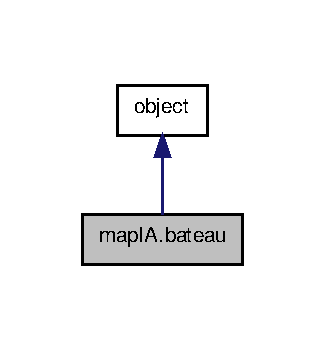
\includegraphics[width=156pt]{classmapIA_1_1bateau__inherit__graph}
\end{center}
\end{figure}


Graphe de collaboration de map\-I\-A.\-bateau\-:
\nopagebreak
\begin{figure}[H]
\begin{center}
\leavevmode
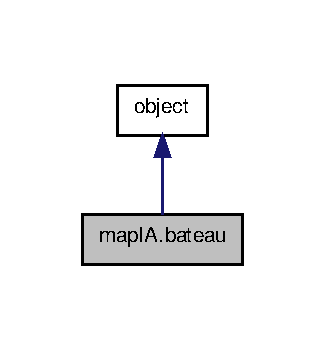
\includegraphics[width=156pt]{classmapIA_1_1bateau__coll__graph}
\end{center}
\end{figure}
\subsection*{Fonctions membres publiques}
\begin{DoxyCompactItemize}
\item 
def \hyperlink{classmapIA_1_1bateau_a2531c2e015fc0ad53bfd1e4e3e1e10e5}{\-\_\-\-\_\-init\-\_\-\-\_\-}
\begin{DoxyCompactList}\small\item\em le constructeur \end{DoxyCompactList}\item 
def \hyperlink{classmapIA_1_1bateau_a4473331f2635b19a588c4cd79cd66546}{\-\_\-\-\_\-str\-\_\-\-\_\-}
\end{DoxyCompactItemize}
\subsection*{Attributs publics}
\begin{DoxyCompactItemize}
\item 
\hyperlink{classmapIA_1_1bateau_a3745885f8dfd7d56a7969309c40d3bf7}{longueur}
\item 
\hyperlink{classmapIA_1_1bateau_ad26a4ff434b6c93397562bd22d8441ef}{sens}
\item 
\hyperlink{classmapIA_1_1bateau_a22b937ab40b572c3a26399362f6a6a25}{originex}
\item 
\hyperlink{classmapIA_1_1bateau_a57b3b7fea3adf6fa95979d8f2f03aa59}{originey}
\item 
\hyperlink{classmapIA_1_1bateau_ad292ca7beb5de446c7ef3c2d1433ed94}{name}
\item 
\hyperlink{classmapIA_1_1bateau_a0a2fc05650b824b75c6652ba33ced801}{pv}
\item 
\hyperlink{classmapIA_1_1bateau_aecb3a9a1d15df3aeac510797e5914054}{statut}
\end{DoxyCompactItemize}


\subsection{Description détaillée}
classe pour impl�menter les bateaux 

Définition à la ligne 40 du fichier map\-I\-A.\-py.



\subsection{Documentation des constructeurs et destructeur}
\hypertarget{classmapIA_1_1bateau_a2531c2e015fc0ad53bfd1e4e3e1e10e5}{\index{map\-I\-A\-::bateau@{map\-I\-A\-::bateau}!\-\_\-\-\_\-init\-\_\-\-\_\-@{\-\_\-\-\_\-init\-\_\-\-\_\-}}
\index{\-\_\-\-\_\-init\-\_\-\-\_\-@{\-\_\-\-\_\-init\-\_\-\-\_\-}!mapIA::bateau@{map\-I\-A\-::bateau}}
\subsubsection[{\-\_\-\-\_\-init\-\_\-\-\_\-}]{\setlength{\rightskip}{0pt plus 5cm}def map\-I\-A.\-bateau.\-\_\-\-\_\-init\-\_\-\-\_\- (
\begin{DoxyParamCaption}
\item[{}]{self, }
\item[{}]{longueur = {\ttfamily 0}, }
\item[{}]{sens = {\ttfamily 0}, }
\item[{}]{originex = {\ttfamily 0}, }
\item[{}]{originey = {\ttfamily 0}, }
\item[{}]{name = {\ttfamily \char`\"{}\char`\"{}}, }
\item[{}]{statut = {\ttfamily \char`\"{}entier\char`\"{}}}
\end{DoxyParamCaption}
)}}\label{classmapIA_1_1bateau_a2531c2e015fc0ad53bfd1e4e3e1e10e5}


le constructeur 


\begin{DoxyParams}{Paramètres}
{\em longueur} & taille du bateau \\
\hline
{\em sens} & 0 vertical et 1 horizontal \\
\hline
{\em originex} & abscisse de la premiere case du bateau \\
\hline
{\em originey} & ordonn�e de la premiere case du bateau \\
\hline
{\em name} & nom du bateau \\
\hline
\end{DoxyParams}


Définition à la ligne 50 du fichier map\-I\-A.\-py.



\subsection{Documentation des fonctions membres}
\hypertarget{classmapIA_1_1bateau_a4473331f2635b19a588c4cd79cd66546}{\index{map\-I\-A\-::bateau@{map\-I\-A\-::bateau}!\-\_\-\-\_\-str\-\_\-\-\_\-@{\-\_\-\-\_\-str\-\_\-\-\_\-}}
\index{\-\_\-\-\_\-str\-\_\-\-\_\-@{\-\_\-\-\_\-str\-\_\-\-\_\-}!mapIA::bateau@{map\-I\-A\-::bateau}}
\subsubsection[{\-\_\-\-\_\-str\-\_\-\-\_\-}]{\setlength{\rightskip}{0pt plus 5cm}def map\-I\-A.\-bateau.\-\_\-\-\_\-str\-\_\-\-\_\- (
\begin{DoxyParamCaption}
\item[{}]{self}
\end{DoxyParamCaption}
)}}\label{classmapIA_1_1bateau_a4473331f2635b19a588c4cd79cd66546}


Définition à la ligne 59 du fichier map\-I\-A.\-py.



\subsection{Documentation des données membres}
\hypertarget{classmapIA_1_1bateau_a3745885f8dfd7d56a7969309c40d3bf7}{\index{map\-I\-A\-::bateau@{map\-I\-A\-::bateau}!longueur@{longueur}}
\index{longueur@{longueur}!mapIA::bateau@{map\-I\-A\-::bateau}}
\subsubsection[{longueur}]{\setlength{\rightskip}{0pt plus 5cm}map\-I\-A.\-bateau.\-longueur}}\label{classmapIA_1_1bateau_a3745885f8dfd7d56a7969309c40d3bf7}


Définition à la ligne 51 du fichier map\-I\-A.\-py.

\hypertarget{classmapIA_1_1bateau_ad292ca7beb5de446c7ef3c2d1433ed94}{\index{map\-I\-A\-::bateau@{map\-I\-A\-::bateau}!name@{name}}
\index{name@{name}!mapIA::bateau@{map\-I\-A\-::bateau}}
\subsubsection[{name}]{\setlength{\rightskip}{0pt plus 5cm}map\-I\-A.\-bateau.\-name}}\label{classmapIA_1_1bateau_ad292ca7beb5de446c7ef3c2d1433ed94}


Définition à la ligne 55 du fichier map\-I\-A.\-py.

\hypertarget{classmapIA_1_1bateau_a22b937ab40b572c3a26399362f6a6a25}{\index{map\-I\-A\-::bateau@{map\-I\-A\-::bateau}!originex@{originex}}
\index{originex@{originex}!mapIA::bateau@{map\-I\-A\-::bateau}}
\subsubsection[{originex}]{\setlength{\rightskip}{0pt plus 5cm}map\-I\-A.\-bateau.\-originex}}\label{classmapIA_1_1bateau_a22b937ab40b572c3a26399362f6a6a25}


Définition à la ligne 53 du fichier map\-I\-A.\-py.

\hypertarget{classmapIA_1_1bateau_a57b3b7fea3adf6fa95979d8f2f03aa59}{\index{map\-I\-A\-::bateau@{map\-I\-A\-::bateau}!originey@{originey}}
\index{originey@{originey}!mapIA::bateau@{map\-I\-A\-::bateau}}
\subsubsection[{originey}]{\setlength{\rightskip}{0pt plus 5cm}map\-I\-A.\-bateau.\-originey}}\label{classmapIA_1_1bateau_a57b3b7fea3adf6fa95979d8f2f03aa59}


Définition à la ligne 54 du fichier map\-I\-A.\-py.

\hypertarget{classmapIA_1_1bateau_a0a2fc05650b824b75c6652ba33ced801}{\index{map\-I\-A\-::bateau@{map\-I\-A\-::bateau}!pv@{pv}}
\index{pv@{pv}!mapIA::bateau@{map\-I\-A\-::bateau}}
\subsubsection[{pv}]{\setlength{\rightskip}{0pt plus 5cm}map\-I\-A.\-bateau.\-pv}}\label{classmapIA_1_1bateau_a0a2fc05650b824b75c6652ba33ced801}


Définition à la ligne 56 du fichier map\-I\-A.\-py.

\hypertarget{classmapIA_1_1bateau_ad26a4ff434b6c93397562bd22d8441ef}{\index{map\-I\-A\-::bateau@{map\-I\-A\-::bateau}!sens@{sens}}
\index{sens@{sens}!mapIA::bateau@{map\-I\-A\-::bateau}}
\subsubsection[{sens}]{\setlength{\rightskip}{0pt plus 5cm}map\-I\-A.\-bateau.\-sens}}\label{classmapIA_1_1bateau_ad26a4ff434b6c93397562bd22d8441ef}


Définition à la ligne 52 du fichier map\-I\-A.\-py.

\hypertarget{classmapIA_1_1bateau_aecb3a9a1d15df3aeac510797e5914054}{\index{map\-I\-A\-::bateau@{map\-I\-A\-::bateau}!statut@{statut}}
\index{statut@{statut}!mapIA::bateau@{map\-I\-A\-::bateau}}
\subsubsection[{statut}]{\setlength{\rightskip}{0pt plus 5cm}map\-I\-A.\-bateau.\-statut}}\label{classmapIA_1_1bateau_aecb3a9a1d15df3aeac510797e5914054}


Définition à la ligne 57 du fichier map\-I\-A.\-py.



La documentation de cette classe a été générée à partir du fichier suivant \-:\begin{DoxyCompactItemize}
\item 
\hyperlink{mapIA_8py}{map\-I\-A.\-py}\end{DoxyCompactItemize}

\hypertarget{classserveur_1_1BatNav}{\section{Référence de la classe serveur.\-Bat\-Nav}
\label{classserveur_1_1BatNav}\index{serveur.\-Bat\-Nav@{serveur.\-Bat\-Nav}}
}


cette classe est la définition d'un service web.  


\subsection*{Fonctions membres publiques}
\begin{DoxyCompactItemize}
\item 
def \hyperlink{classserveur_1_1BatNav_a4bee30dcf9c6439b0120b0f84e351c8e}{check\-Session}
\begin{DoxyCompactList}\small\item\em crée un cookie de session si celui-\/ci n'existe pas encore ; enregistre l'heure de début et procède à une authentification, si nécesaire. \end{DoxyCompactList}\item 
def \hyperlink{classserveur_1_1BatNav_a788dcf39ae9210eece7d5a1ee4ea593e}{index}
\begin{DoxyCompactList}\small\item\em page racine du site web. \end{DoxyCompactList}\item 
def \hyperlink{classserveur_1_1BatNav_afb6d70a94f46205136428435bffdc442}{login}
\begin{DoxyCompactList}\small\item\em demande le nom et le stocke dans la session \end{DoxyCompactList}\item 
def \hyperlink{classserveur_1_1BatNav_a2e39322808163b8d156562e198518ccf}{jeu}
\begin{DoxyCompactList}\small\item\em Cette page sert à renvoyer au format J\-S\-O\-N un certain nombre de données organisées en dictionnaire Python. \end{DoxyCompactList}\item 
def \hyperlink{classserveur_1_1BatNav_a88cb8ae9a230bca42163914af847774c}{Init}
\begin{DoxyCompactList}\small\item\em Cette page permet à l'utilisateur de positionner ses bateaux. \end{DoxyCompactList}\item 
def \hyperlink{classserveur_1_1BatNav_ab071e379cd4ee3eecce78dbe29e42781}{combat}
\begin{DoxyCompactList}\small\item\em Cette page permet à l'utilisateur de jouer contre l'I\-A. \end{DoxyCompactList}\item 
def \hyperlink{classserveur_1_1BatNav_a3a8c5179e629add650e9472e9759e3e3}{arthur}
\begin{DoxyCompactList}\small\item\em Cette page sert à renvoyer au format J\-S\-O\-N un certain nombre de données organisées en dictionnaire Python. \end{DoxyCompactList}\end{DoxyCompactItemize}


\subsection{Description détaillée}
cette classe est la définition d'un service web. 

Les méthodes dont l'attribut exposed est Vrai sont autant de pages servies par le serveur web. 

Définition à la ligne 34 du fichier serveur.\-py.



\subsection{Documentation des fonctions membres}
\hypertarget{classserveur_1_1BatNav_a3a8c5179e629add650e9472e9759e3e3}{\index{serveur\-::\-Bat\-Nav@{serveur\-::\-Bat\-Nav}!arthur@{arthur}}
\index{arthur@{arthur}!serveur::BatNav@{serveur\-::\-Bat\-Nav}}
\subsubsection[{arthur}]{\setlength{\rightskip}{0pt plus 5cm}def serveur.\-Bat\-Nav.\-arthur (
\begin{DoxyParamCaption}
\item[{}]{self, }
\item[{}]{dico}
\end{DoxyParamCaption}
)}}\label{classserveur_1_1BatNav_a3a8c5179e629add650e9472e9759e3e3}


Cette page sert à renvoyer au format J\-S\-O\-N un certain nombre de données organisées en dictionnaire Python. 


\begin{DoxyParams}{Paramètres}
{\em dico} & dictionnaire contenant les variables \\
\hline
\end{DoxyParams}


Définition à la ligne 206 du fichier serveur.\-py.

\hypertarget{classserveur_1_1BatNav_a4bee30dcf9c6439b0120b0f84e351c8e}{\index{serveur\-::\-Bat\-Nav@{serveur\-::\-Bat\-Nav}!check\-Session@{check\-Session}}
\index{check\-Session@{check\-Session}!serveur::BatNav@{serveur\-::\-Bat\-Nav}}
\subsubsection[{check\-Session}]{\setlength{\rightskip}{0pt plus 5cm}def serveur.\-Bat\-Nav.\-check\-Session (
\begin{DoxyParamCaption}
\item[{}]{self}
\end{DoxyParamCaption}
)}}\label{classserveur_1_1BatNav_a4bee30dcf9c6439b0120b0f84e351c8e}


crée un cookie de session si celui-\/ci n'existe pas encore ; enregistre l'heure de début et procède à une authentification, si nécesaire. 



Définition à la ligne 41 du fichier serveur.\-py.

\hypertarget{classserveur_1_1BatNav_ab071e379cd4ee3eecce78dbe29e42781}{\index{serveur\-::\-Bat\-Nav@{serveur\-::\-Bat\-Nav}!combat@{combat}}
\index{combat@{combat}!serveur::BatNav@{serveur\-::\-Bat\-Nav}}
\subsubsection[{combat}]{\setlength{\rightskip}{0pt plus 5cm}def serveur.\-Bat\-Nav.\-combat (
\begin{DoxyParamCaption}
\item[{}]{self, }
\item[{}]{dico}
\end{DoxyParamCaption}
)}}\label{classserveur_1_1BatNav_ab071e379cd4ee3eecce78dbe29e42781}


Cette page permet à l'utilisateur de jouer contre l'I\-A. 


\begin{DoxyParams}{Paramètres}
{\em dico} & dictionnaire contenant toutes les variables \\
\hline
\end{DoxyParams}


Définition à la ligne 177 du fichier serveur.\-py.

\hypertarget{classserveur_1_1BatNav_a788dcf39ae9210eece7d5a1ee4ea593e}{\index{serveur\-::\-Bat\-Nav@{serveur\-::\-Bat\-Nav}!index@{index}}
\index{index@{index}!serveur::BatNav@{serveur\-::\-Bat\-Nav}}
\subsubsection[{index}]{\setlength{\rightskip}{0pt plus 5cm}def serveur.\-Bat\-Nav.\-index (
\begin{DoxyParamCaption}
\item[{}]{self}
\end{DoxyParamCaption}
)}}\label{classserveur_1_1BatNav_a788dcf39ae9210eece7d5a1ee4ea593e}


page racine du site web. 

\begin{DoxyReturn}{Renvoie}
une page web qui devrait être valide pour le W3\-C. Cette page décrit brièvement le jeu de bataille navale et permet de commencer à jouer. 
\end{DoxyReturn}


Définition à la ligne 57 du fichier serveur.\-py.

\hypertarget{classserveur_1_1BatNav_a88cb8ae9a230bca42163914af847774c}{\index{serveur\-::\-Bat\-Nav@{serveur\-::\-Bat\-Nav}!Init@{Init}}
\index{Init@{Init}!serveur::BatNav@{serveur\-::\-Bat\-Nav}}
\subsubsection[{Init}]{\setlength{\rightskip}{0pt plus 5cm}def serveur.\-Bat\-Nav.\-Init (
\begin{DoxyParamCaption}
\item[{}]{self, }
\item[{}]{dico}
\end{DoxyParamCaption}
)}}\label{classserveur_1_1BatNav_a88cb8ae9a230bca42163914af847774c}


Cette page permet à l'utilisateur de positionner ses bateaux. 


\begin{DoxyParams}{Paramètres}
{\em dico} & dictionnaire contenant toutes les variables \\
\hline
\end{DoxyParams}


Définition à la ligne 146 du fichier serveur.\-py.

\hypertarget{classserveur_1_1BatNav_a2e39322808163b8d156562e198518ccf}{\index{serveur\-::\-Bat\-Nav@{serveur\-::\-Bat\-Nav}!jeu@{jeu}}
\index{jeu@{jeu}!serveur::BatNav@{serveur\-::\-Bat\-Nav}}
\subsubsection[{jeu}]{\setlength{\rightskip}{0pt plus 5cm}def serveur.\-Bat\-Nav.\-jeu (
\begin{DoxyParamCaption}
\item[{}]{self, }
\item[{}]{dico}
\end{DoxyParamCaption}
)}}\label{classserveur_1_1BatNav_a2e39322808163b8d156562e198518ccf}


Cette page sert à renvoyer au format J\-S\-O\-N un certain nombre de données organisées en dictionnaire Python. 

La conversion au format J\-S\-O\-N est faite automatiquement par le module Cherrypy, grâce au \char`\"{}décorateur\char`\"{} cherrypy.\-tools.\-json\-\_\-out() 
\begin{DoxyParams}{Paramètres}
{\em dico} & le dictionnaire qui rassemble les données entrantes. ces données sont celles que la page reçoit. \\
\hline
\end{DoxyParams}
\begin{DoxyReturn}{Renvoie}
un objet au format J\-S\-O\-N, ses champs doivent être explicites. 
\end{DoxyReturn}


Définition à la ligne 121 du fichier serveur.\-py.

\hypertarget{classserveur_1_1BatNav_afb6d70a94f46205136428435bffdc442}{\index{serveur\-::\-Bat\-Nav@{serveur\-::\-Bat\-Nav}!login@{login}}
\index{login@{login}!serveur::BatNav@{serveur\-::\-Bat\-Nav}}
\subsubsection[{login}]{\setlength{\rightskip}{0pt plus 5cm}def serveur.\-Bat\-Nav.\-login (
\begin{DoxyParamCaption}
\item[{}]{self, }
\item[{}]{url\-\_\-retour = {\ttfamily \char`\"{}/Init\char`\"{}}, }
\item[{}]{dico}
\end{DoxyParamCaption}
)}}\label{classserveur_1_1BatNav_afb6d70a94f46205136428435bffdc442}


demande le nom et le stocke dans la session 


\begin{DoxyParams}{Paramètres}
{\em url\-\_\-retour} & est l'U\-R\-L à servir dès que le nom est défini. url\-\_\-retour est la racine du site par défaut. \\
\hline
{\em dico} & dictionnaire des paramètres envoyés, par le formulaire, ou à partir d'une autre page. Si la clé \char`\"{}nom\char`\"{} correspond à une valeur, celle-\/ci sera utilisée pour le login. \\
\hline
\end{DoxyParams}
\begin{DoxyReturn}{Renvoie}
un formulaire pour l'authentification si celle-\/ci n'est pas définie dans le dictionnaire dico. Sinon ne renvoie rien \-: un mécanisme d'exception déclenche le service de la page web désignée par url\-\_\-retour. 
\end{DoxyReturn}


Définition à la ligne 89 du fichier serveur.\-py.



La documentation de cette classe a été générée à partir du fichier suivant \-:\begin{DoxyCompactItemize}
\item 
\hyperlink{serveur_8py}{serveur.\-py}\end{DoxyCompactItemize}

\hypertarget{classobject}{\section{Référence de la classe object}
\label{classobject}\index{object@{object}}
}


Graphe d'héritage de object\-:
\nopagebreak
\begin{figure}[H]
\begin{center}
\leavevmode
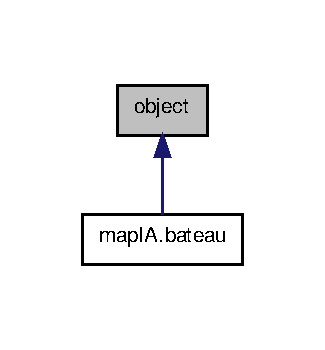
\includegraphics[width=156pt]{classobject__inherit__graph}
\end{center}
\end{figure}


La documentation de cette classe a été générée à partir du fichier suivant \-:\begin{DoxyCompactItemize}
\item 
\hyperlink{mapIA_8py}{map\-I\-A.\-py}\end{DoxyCompactItemize}

\chapter{Documentation des fichiers}
\hypertarget{bateau_8py}{\section{Référence du fichier bateau.\-py}
\label{bateau_8py}\index{bateau.\-py@{bateau.\-py}}
}
\subsection*{Espaces de nommage}
\begin{DoxyCompactItemize}
\item 
\hyperlink{namespacebateau}{bateau}
\end{DoxyCompactItemize}
\subsection*{Fonctions}
\begin{DoxyCompactItemize}
\item 
def \hyperlink{namespacebateau_a2f0e2fb6690af90fd1cd510e132a041c}{bateau.\-map}
\item 
def \hyperlink{namespacebateau_ad2ef327d271e5ebe5426fe6d58fa0cea}{bateau.\-Porte\-Avion}
\item 
def \hyperlink{namespacebateau_a472c5b7bcdfb78f0e7388a197a25129a}{bateau.\-Croiseur}
\item 
def \hyperlink{namespacebateau_a91714c8dcf7e649256b4abd289176d58}{bateau.\-Contre\-Torpilleur}
\item 
def \hyperlink{namespacebateau_ae08b97eef04ed71124cda74053ad0a36}{bateau.\-Sous\-Marin}
\item 
def \hyperlink{namespacebateau_a875c36de98747c833df6a8c648f0ced3}{bateau.\-Torpilleur}
\item 
def \hyperlink{namespacebateau_aa9dece4300bcd47e6e67cdaa52fa2cce}{bateau.\-sens}
\item 
def \hyperlink{namespacebateau_ad1217acc7738157178dae5d246b019db}{bateau.\-originex}
\item 
def \hyperlink{namespacebateau_a2b16dc7153e94407fdbb3c8d4a152a84}{bateau.\-originey}
\end{DoxyCompactItemize}
\subsection*{Variables}
\begin{DoxyCompactItemize}
\item 
tuple \hyperlink{namespacebateau_a924cee8dc4435fc03e905904c31dbcf7}{bateau.\-Carte\-Joueur} = map()
\item 
tuple \hyperlink{namespacebateau_a50dc5f1cd8aae1c80cfd24007c44dd9c}{bateau.\-Carte\-Adv} = map()
\end{DoxyCompactItemize}

\hypertarget{constantes_8py}{\section{Référence du fichier constantes.\-py}
\label{constantes_8py}\index{constantes.\-py@{constantes.\-py}}
}


Copyright (c) 2014 Georges Khaznadar \href{mailto:georgesk@debian.org}{\tt georgesk@debian.\-org}  


\subsection*{Espaces de nommage}
\begin{DoxyCompactItemize}
\item 
\hyperlink{namespaceconstantes}{constantes}
\end{DoxyCompactItemize}
\subsection*{Variables}
\begin{DoxyCompactItemize}
\item 
string \hyperlink{namespaceconstantes_a04524e30f424889c8a4407e02f93755f}{constantes.\-H\-T\-M\-L\-\_\-header}
\begin{DoxyCompactList}\small\item\em Début du fichier H\-T\-M\-L; définit précisément le format utilisé, pour la conformité à la norme stricte du W3\-C. \end{DoxyCompactList}\item 
string \hyperlink{namespaceconstantes_a43ef8a067f33f666e58da77fae47ecd4}{constantes.\-H\-T\-M\-L\-\_\-footer}
\item 
string \hyperlink{namespaceconstantes_aa2fb1d8038db179e532f06a5e7bb578b}{constantes.\-H\-T\-M\-L\-\_\-script\-Init}
\item 
string \hyperlink{namespaceconstantes_a4bd1e6c18ef13d98f076c27d0e463532}{constantes.\-H\-T\-M\-L\-\_\-script\-Authen}
\item 
string \hyperlink{namespaceconstantes_a98851e65f9b7b6f42bd22f328e548889}{constantes.\-H\-T\-M\-L\-\_\-script\-Combat}
\end{DoxyCompactItemize}


\subsection{Description détaillée}
Copyright (c) 2014 Georges Khaznadar \href{mailto:georgesk@debian.org}{\tt georgesk@debian.\-org} Ce fichier fait partie du projet Batnav Batnav est un petit logiciel libre, vous avez le droit de le réutiliser à votre convenance, dans le respect de la licence G\-P\-L V3, ou, selon vos préférences, de toute version ultérieure de celle-\/ci. Le texte de la licence est disponible à \href{http://www.gnu.org/licenses/gpl.html}{\tt http\-://www.\-gnu.\-org/licenses/gpl.\-html} 

Définition dans le fichier \hyperlink{constantes_8py_source}{constantes.\-py}.


\hypertarget{mapIA_8py}{\section{Référence du fichier map\-I\-A.\-py}
\label{mapIA_8py}\index{map\-I\-A.\-py@{map\-I\-A.\-py}}
}


Ce fichier fait partie du projet Batnav Batnav est un petit logiciel libre, vous avez le droit de le r�utiliser � votre convenance, dans le respect de la licence G\-P\-L V3, ou, selon vos pr�f�rences, de toute version ult�rieure de celle-\/ci.  


\subsection*{Classes}
\begin{DoxyCompactItemize}
\item 
class \hyperlink{classmapIA_1_1bateau}{map\-I\-A.\-bateau}
\begin{DoxyCompactList}\small\item\em classe pour impl�menter les bateaux \end{DoxyCompactList}\end{DoxyCompactItemize}
\subsection*{Espaces de nommage}
\begin{DoxyCompactItemize}
\item 
\hyperlink{namespacemapIA}{map\-I\-A}
\end{DoxyCompactItemize}
\subsection*{Fonctions}
\begin{DoxyCompactItemize}
\item 
def \hyperlink{namespacemapIA_a07aa7cef6cded245e3726ca002ada4cc}{map\-I\-A.\-map}
\begin{DoxyCompactList}\small\item\em Initialisation de terrain de jeu vide. \end{DoxyCompactList}\item 
def \hyperlink{namespacemapIA_acaa6e2766241424eab25926347449709}{map\-I\-A.\-utilisateur}
\begin{DoxyCompactList}\small\item\em permet de d�finir la carte de jeu du joueur \end{DoxyCompactList}\item 
def \hyperlink{namespacemapIA_aa3e6bde576e412f528beeb2a4284610e}{map\-I\-A.\-ordi}
\begin{DoxyCompactList}\small\item\em permet de d�finir une carte al�atoire \end{DoxyCompactList}\item 
def \hyperlink{namespacemapIA_a879cad271640caa500dfe0a71afdaa11}{map\-I\-A.\-init}
\begin{DoxyCompactList}\small\item\em permet de transformer un dictionnaire python contenant des positions de bateaux en une liste \end{DoxyCompactList}\end{DoxyCompactItemize}
\subsection*{Variables}
\begin{DoxyCompactItemize}
\item 
list \hyperlink{namespacemapIA_a2eb569dd5a95aebd189ad07e5780dfc7}{map\-I\-A.\-utilise} = \mbox{[}$\,$\mbox{]}
\item 
list \hyperlink{namespacemapIA_a309a59b71877fe3d9646b1ca13e6da99}{map\-I\-A.\-utilise\-I\-A} = \mbox{[}$\,$\mbox{]}
\item 
tuple \hyperlink{namespacemapIA_a31fc24195ea636531e2a0f87535e8584}{map\-I\-A.\-Porte\-Avion} = bateau(longueur=5,name=\char`\"{}Porte avion\char`\"{})
\item 
tuple \hyperlink{namespacemapIA_a9b0b78e5b10e3c69824c980e804d8e3a}{map\-I\-A.\-Croiseur} = bateau(longueur=4,name=\char`\"{}Croiseur\char`\"{})
\item 
tuple \hyperlink{namespacemapIA_a328579f1726b839070a7447c1aaa1dc4}{map\-I\-A.\-Contre\-Torpilleur} = bateau(longueur=3,name=\char`\"{}Contre-\/torpilleur\char`\"{})
\item 
tuple \hyperlink{namespacemapIA_a9b5c834a25a2fec1c150226e63acb189}{map\-I\-A.\-Sous\-Marin} = bateau(longueur=3,name=\char`\"{}Sous marin\char`\"{})
\item 
tuple \hyperlink{namespacemapIA_a3ff6b55b368579554153d76cb8b40752}{map\-I\-A.\-Torpilleur1} = bateau(longueur=2,name=\char`\"{}Torpilleur 1\char`\"{})
\item 
tuple \hyperlink{namespacemapIA_a53be1d89da79a45d9abc4e7ee4d26686}{map\-I\-A.\-Torpilleur2} = bateau(longueur=2,name=\char`\"{}Torpilleur 2\char`\"{})
\item 
tuple \hyperlink{namespacemapIA_a2f95e844f52fe35f954ce1b15bf78c28}{map\-I\-A.\-Carte\-Joueur} = map()
\item 
tuple \hyperlink{namespacemapIA_a8dc9582830d71f060d8803eddabecfa8}{map\-I\-A.\-Carte\-I\-A} = map()
\item 
list \hyperlink{namespacemapIA_af66becab7592d928fa0ff7a4af6431c8}{map\-I\-A.\-l} = \mbox{[}Porte\-Avion,Croiseur,Contre\-Torpilleur,Sous\-Marin,Torpilleur1,Torpilleur2\mbox{]}
\end{DoxyCompactItemize}


\subsection{Description détaillée}
Ce fichier fait partie du projet Batnav Batnav est un petit logiciel libre, vous avez le droit de le r�utiliser � votre convenance, dans le respect de la licence G\-P\-L V3, ou, selon vos pr�f�rences, de toute version ult�rieure de celle-\/ci. Le texte de la licence est disponible � \href{http://www.gnu.org/licenses/gpl.html}{\tt http\-://www.\-gnu.\-org/licenses/gpl.\-html} 

Définition dans le fichier \hyperlink{mapIA_8py_source}{map\-I\-A.\-py}.


\hypertarget{serveur_8py}{\section{Référence du fichier serveur.\-py}
\label{serveur_8py}\index{serveur.\-py@{serveur.\-py}}
}
\subsection*{Classes}
\begin{DoxyCompactItemize}
\item 
class \hyperlink{classserveur_1_1BatNav}{serveur.\-Bat\-Nav}
\begin{DoxyCompactList}\small\item\em cette classe est la définition d'un service web. \end{DoxyCompactList}\end{DoxyCompactItemize}
\subsection*{Espaces de nommage}
\begin{DoxyCompactItemize}
\item 
\hyperlink{namespaceserveur}{serveur}
\end{DoxyCompactItemize}
\subsection*{Constant Groups}
\begin{DoxyCompactItemize}
\item 
\hyperlink{namespaceserveur}{serveur}
\end{DoxyCompactItemize}
\subsection*{Variables}
\begin{DoxyCompactItemize}
\item 
tuple \hyperlink{namespaceserveur_a67de12cb5d8d1fc1b938786191e6e7a3}{serveur.\-\_\-\-S\-T\-A\-T\-I\-C\-\_\-\-D\-I\-R} = os.\-path.\-join(os.\-path.\-abspath(\char`\"{}.\char`\"{}), \char`\"{}static\char`\"{})
\item 
dictionary \hyperlink{namespaceserveur_ab0d89e80607d8c3e353fbdec568c25c1}{serveur.\-dev\-\_\-config}
\end{DoxyCompactItemize}

%--- End generated contents ---

% Index
\newpage
\phantomsection
\addcontentsline{toc}{chapter}{Index}
\printindex

\end{document}
